% ch6.tex
% Dieses Werk ist unter einem Creative Commons Namensnennung-Keine kommerzielle Nutzung-Weitergabe
% unter gleichen Bedingungen 3.0 Deutschland Lizenzvertrag lizenziert. Um die Lizenz anzusehen, gehen Sie bitte
% zu http://creativecommons.org/licenses/by-nc-sa/3.0/de/ oder schicken Sie einen Brief an
% Creative Commons, 171 Second Street, Suite 300, San Francisco, California 94105, USA.


%\chapter{Sort of like recycling$\ldots$}\label{ch:sortoflikerecycling}
\chapter{Wie Recycling$\ldots$}\label{ch:sortoflikerecycling}

%Think about how much rubbish you create each day. Bottled water or bottles of soft drink, packets of crisps, plastic sandwich wrappers, bags of vegetables, meat on plastic trays, plastic shopping bags, newspapers, magazines, and so on and so on and so on$\ldots$
Denke einmal darüber nach, wie viel Müll du jeden Tag erzeugst. Getränkeflaschen, Chipstüten, Sandwichpapier, Fleischtassen, Einkaufstüten, Zeitungen, Magazine und so weiter.
\par
%Now just think about what would happen if all of that trash just got dumped in a pile at the end of your driveway.
Stell dir einmal kurz vor wie das wäre, wenn der ganze Müll am Ende deiner Straße auf einen großen Haufen landen würde.

\begin{center}
\includegraphics*[width=100mm]{images/trash}
\end{center}

%Of course, you probably recycle as much as possible.  Which is fortunate, because no one likes having to climb over a rubbish heap, on the way to school.  So, those glass bottles in the recycle bin are hopefully melted down, and then turned into new jars and bottles; paper is pulped into recycled paper; plastic turned into heavier plastic goods---so your front lawn doesn't disappear under tonnes of garbage. We get to reuse some of the goods we create, rather than eating a gaping hole in the side of the world to manufacture the same things over and over again.
Vielleicht trennst du jetzt schon den Müll und hilfst so bei der Wiederverwertung. Das ist auch ein Glück, denn niemand will gerne auf dem Weg in die Schule über einen Müllberg klettern. Mit dem Recycling werden aus alten Glasflaschen wieder neue. Aus Plastik neuer Kunststoff und aus Altpapier werden wieder neue Zeitungen.

%Recycling or reuse, in the programming world, is just as important. Not because your program will disappear under a pile of garbage---but if you don't re-use some of what you're doing, you'll eventually wear your fingers down to painful stubs through over-typing.
Recycling und Wiederverwerten sind in der Welt der Programmierung genauso interessant. Nicht weil dein Programm unter einem Müllberg verschwinden würde---sondern damit du deine Fingerkuppen schonst, und nicht alles immer wieder eintippen musst.

%There are a number of different ways to reuse code in Python (and in programming languages in general), but we've seen one of the ways already, back in Chapter 3, with the function range.  Functions\index{functions} are one way to reuse code---so you can write the code once, then use it in your programs again and again.  Let's first try a simple example of a function:
Es gibt verschiedene Möglichkeiten in Python (und anderen Programmiersprachen) wie man Code wieder verwendet, und eine Art haben wir schon in Kapitel 3 mit der range Funktion kennengelernt. Funktionen\index{Funktionen} sind also eine Art der Wiederverwendung---du schreibst den Code einmal und verwendest ihn in deinem Programmen immer wieder. Probier ein einfaches Beispiel:

%\begin{listing}
%\begin{verbatim}
%>>> def myfunction(myname):
%...     print('hello %s' % myname)
%...
%\end{verbatim}
%\end{listing}
\begin{Verbatim}[frame=single]
>>> def meine_funktion(mein_name):
...     print('Hallo %s' % mein_name)
...
\end{Verbatim}


%The above function has a name `myfunction' and has a parameter `myname'.  A \emph{parameter} is a variable which is only available within the `body' of the function (which is the block of code immediately after the line starting with \code{def}---in case you're wondering, \code{def} is short for define).  You can run the function by calling its name with brackets surrounding the parameter value:
Diese Funktion hat den Namen `meine\_funktion' und hat den Parameter `mein\_name'. Ein \emph{Parameter} ist eine Variable, die nur innerhalb eines Blockes eine Bedeutung hat (das ist der Block der sofort nach der \code{def} Zeile beginnt). \code{def} ist die Kurzform von define und mit diesem Schlüsselwort definierst du Funktionen. Die Funktion kannst du ausprobieren, indem du sie aufrufst und in runden Klammern einen Parameter mitgibst.

%\begin{listing}
%\begin{verbatim}
%>>> myfunction('Mary')
%hello Mary
%\end{verbatim}
%\end{listing}
\begin{Verbatim}[frame=single]
>>> meine_funktion('Hannah')
Hallo Hannah
\end{Verbatim}


\noindent
%We could change the function to take 2 parameters:
Jetzt ändern wir die Funktion, damit 2 Parameter übergeben werden können:

%\begin{listing}
%\begin{verbatim}
%>>> def myfunction(firstname, lastname):
%...     print('Hello %s %s' % (firstname, lastname))
%...
%\end{verbatim}
%\end{listing}
\begin{Verbatim}[frame=single]
>>> def meine_funktion(vorname, nachname):
...     print('Hallo %s %s' % (vorname, nachname))
...
\end{Verbatim}

\noindent
%And then call it in a similar fashion to the first:
Und aufrufen funktioniert ganz ähnlich:

%\begin{listing}
%\begin{verbatim}
%>>> myfunction('Mary', 'Smith')
%Hello Mary Smith
%\end{verbatim}
%\end{listing}
\begin{Verbatim}[frame=single]
>>> meine_funktion('Hannah', 'Schmidt')
Hallo Hanna Schmidt
\end{Verbatim}

\noindent
%Or we could create some variables and call the function with the variables:
Oder wir erzeugen ein Paar Variablen und rufen die Funktion mit den Variablen auf:

%\begin{listing}
%\begin{verbatim}
%>>> fn = 'Joe'
%>>> ln = 'Robertson'
%>>> myfunction(fn, ln)
%Hello Joe Robertson
%\end{verbatim}
%\end{listing}
\begin{Verbatim}[frame=single]
>>> vn = 'Tom'
>>> nn = 'Turbo'
>>> meine_funktion(vn, nn)
Hallo Tom Turbo
\end{Verbatim}

\noindent
%We can return values from a function using the \code{return}\index{return} statement:
Und eine Funktion kann auch Werte zurückgeben indem das \code{return}\index{Funktionen!return} Schlüsselwort verwendet wird:

%\begin{Verbatim}[frame=single]
%>>> def savings(chores, paper, spending):
%...     return chores + paper - spending
%...
%>>> print(savings(10, 10, 5))
%15
%\end{Verbatim}
\begin{Verbatim}[frame=single]
>>> def ersparnisse(hausarbeit, zeitung, ausgaben):
...     return hausarbeit + zeitung - ausgaben
...
>>> print(ersparnisse(10, 10, 5))
15
\end{Verbatim}

%This function takes 3 parameters, and then adds the first two (\code{chores} and \code{paper}) before subtracting the last one (\code{spending}).  The result is then returned---this result can be used as the value of a variable (the same way we set other values to variables):
Diese Funktion nimmt 3 Parameter und addiert die ersten zwei (\code{hausarbeit} und \code{zeitung}) bevor es dann den letzten Parameter (\code{ausgaben}) abzieht. Das Ergebnis wird zurückgegeben---und kann wie der Wert einer Variable verwendet werden:

%\begin{Verbatim}[frame=single]
%>>> my_savings = savings(20, 10, 5)
%>>> print(my_savings)
%25
%\end{Verbatim}
\begin{Verbatim}[frame=single]
>>> meine_ersparnisse = ersparnisse(20, 10, 5)
>>> print(meine_ersparnisse)
25
\end{Verbatim}

\noindent
%However, a variable that we use inside the body of a function will not be accessible (usable), when the function has finished:
Variablen, die innerhalb der Funktion verwendet werden, können aber von ausserhalb nicht angesprochen werden.

%\begin{Verbatim}[frame=single]
%>>> def variable_test():
%...     a = 10
%...     b = 20
%...     return a * b
%...
%>>> print(variable_test())
%200
%>>> print(a)
%Traceback (most recent call last):
%  File "<stdin>", line 1, in <module>
%NameError: name 'a' is not defined
%\end{Verbatim}
\begin{Verbatim}[frame=single]
>>> def variable_test():
...     a = 10
...     b = 20
...     return a * b
...
>>> print(variable_test())
200
>>> print(a)
Traceback (most recent call last):
  File "<stdin>", line 1, in <module>
NameError: name 'a' is not defined
\end{Verbatim}

%In the above example we create a function \code{variable\_test}, which multiplies two variables (\code{a} and \code{b}) and returns the result.  If we call this function using \code{print}, we get the answer: 200.  However if we try to print the contents of \code{a} (or \code{b} for that matter), we get the error message ```a' is not defined''. This is something called `\emph{scope}'\index{scope}, in the world of programming.
Im obigen Beispiel erzeugen wir eine Funktion \code{varialbe\_test}, in der zwei Variablen miteinander multipliziert werden (\code{a} und \code{b}) und das Ergebnis wird zurückgegeben. Wenn wir die Funktion mit der \code{print} Funktion aufrufen, bekommen wir 200. Wenn wir aber direkt auf die Variable \code{a} oder \code{b} zugreifen, bekommen wir den Fehler, dass ```a' nicht definiert ist''. In der Programmierwelt wird dieses Verhalten mit dem Begriff `\emph{scope}'\index{Funktionen!scope} erklärt. 
\par
%Think of a function as a little island floating in the ocean---and it's too far to swim from the island to anywhere else.  Occasionally, a plane flies over and drops bits of paper on the island (those are parameters coming into a function) which the inhabitants then stick together into a message, put the message into a bottle and then toss the bottle into the sea (this is the return value).  What the islanders do on the island, and how many of them it took to make the message, makes no difference to the person picking up the bottle and reading the message inside.  This is probably the easiest way to think about scope---but there is one small problem with that idea.  One of the islanders has a large pair of binoculars and can see all the way to the mainland.  He can see what other people are doing there, and that can affect the message that they're creating:
So eine Funktion ist ein wenig wie eine Insel mitten im Ozean. Es ist viel zu weit um von der Insel wegschwimmen zu können. Manchmal fliegt ein Flugzeug über die Insel und wirft Papierzettel mit Nachrichten ab (das sind die Parameter, die in die Funktion übernommen werden). Die Bewohner der Insel kommen zusammen um die Nachrichten zu lesen und stecken die Antwort darauf in eine Flasche, die als Flaschenpost in den Ozean geworfen wird (das ist der Rückgabewert). Was die Eingeborenen auf der Insel machen und wieviele es genau sind, ist für die Person, die die Flaschenpost öffnet nicht von Bedeutung. Das ist wahrscheinlich die einfachste Art \code{scope} zu erklären---bis auf ein kleines wichtiges Detail. Einer der Inselbewohner hat ein großes Fernglas und kann bis aufs Festland schauen. Da sieht er, was die anderen Leute so machen und das kann die Antwort in der Flaschenpost auch beeinflussen.

%\begin{Verbatim}[frame=single]
%>>> x = 100
%>>> def variable_test2():
%...     a = 10
%...     b = 20
%...     return a * b * x
%...
%>>> print(variable_test2())
%20000
%\end{Verbatim}
\begin{Verbatim}[frame=single]
>>> x = 100
>>> def variable_test2():
...     a = 10
...     b = 20
...     return a * b * x
...
>>> print(variable_test2())
20000
\end{Verbatim}

%So, even though variables \code{a} and \code{b} aren't able to be used outside of the function, the variable \code{x} (which was created outside the function) is usable inside.  Just think about the islander with the binoculars, and hopefully it might help that idea to make a little bit of sense.
Obwohl die Variablen \code{a} und \code{b} nicht ausserhalb der Funktion sichtbar sind, kann die Variable \code{x} (die ausserhalb der Funktion erzeugt wurde) innerhalb der Funktion verwendet werden. Denke an den Inselbewohner mit dem Fernglas und vielleicht tust du dir dann leichter.

\begin{center}
\includegraphics*[width=100mm]{images/islanders}
\end{center}

%The for-loop we created earlier to display savings over a year, could easily be added to a function:
Um die Schleife aus dem vorigen Kapitel (mit den Ersparnissen über das Jahr) darzusellen, kann praktischerweise eine Funktion verwendet werden.

%\begin{Verbatim}[frame=single]
%>>> def yearly_savings(chores, paper, spending):
%...     savings = 0
%...     for week in range(1, 53):
%...         savings = savings + chores + paper - spending
%...         print('Week %s = %s' % (week, savings))
%...
%\end{Verbatim}
\begin{Verbatim}[frame=single]
>>> def jahres_ersparnisse(hausarbeit, zeitung, ausgaben):
...     ersparnisse = 0
...     for woche in range(1, 53):
...         ersparnisse = ersparnisse + hausarbeit + zeitung - ausgaben
...         print('Woche %s = %s' % (woche, ersparnisse))
...
\end{Verbatim}

%Try entering that function in the console, and call it with different values for \code{chores}, \code{paper} and \code{spending}:
Gib die Funktion in die Konsole ein und rufe sie mit verschiedenen Werten für \code{hausarbeit}, \code{zeitung} und \code{ausgaben} auf:

%\begin{Verbatim}[frame=single]
%>>> yearly_savings(10, 10, 5)
%Week 1 = 15
%Week 2 = 30
%Week 3 = 45
%Week 4 = 60
%Week 5 = 75
%Week 6 = 90
%Week 7 = 105
%Week 8 = 120
%Week 9 = 135
%Week 10 = 150

%(continues on...)

%>>> yearly_savings(25, 15, 10)
%Week 1 = 30
%Week 2 = 60
%Week 3 = 90
%Week 4 = 120
%Week 5 = 150

%(continues on...)
%\end{Verbatim}
\begin{Verbatim}[frame=single, label=Ausgabe]
>>> jahres_ersparnisse(10, 10, 5)
Woche 1 = 15
Woche 2 = 30
Woche 3 = 45
Woche 4 = 60
Woche 5 = 75
Woche 6 = 90
Woche 7 = 105
Woche 8 = 120
Woche 9 = 135
Woche 10 = 150
Woche 11 = 165

(geht so weiter...)

>>> jahres_ersparnisse(25, 15, 10)
Woche 1 = 30
Woche 2 = 60
Woche 3 = 90
Woche 4 = 120
Woche 5 = 150

(continues on...)
\end{Verbatim}

%This is a bit more useful than re-typing the for-loop every time you want to try it with a different value. Functions can also be grouped together into something called `modules', which is where Python becomes really useful$\ldots$ as opposed to just mildly useful.
Das ist doch schon schöner, als die ganze for-Schleife immer wieder neu zu tippen, wenn du neue Werte übergeben willst. Mehrer Gruppen können auch in sogenanne `Module' zusammengefasst werden und da bringt Python schon so viel mit, dass es wirklich sehr nützlich wird.
\par
\noindent
%\emph{More about modules shortly.}
\emph{Mehr über Module etwas später.}

%\section{Bits and Pieces}
\section{Dies und das} 

%When Python is installed on your computer, a whole pile of functions and modules are also installed. Some functions are available by default.  \code{range} is a function we've already seen. \code{file}\index{functions!file} is another function we haven't use yet.
Wenn Python an deinem Computer installiert wird, wird auch ein ganzer Haufen von Funktionen und Modulen mit installiert. Einige Funktionen sind sofort verfügbar so wie \code{range}. Andere Funktionen so wie \code{file}\index{Funktionen!Datei} auch, aber das haben wir noch nicht verwendet.

\begin{WINDOWS}
%To see how \code{file} is used, open Notepad and type a few words, then save the file onto your C drive, by:
Um zu sehen wie du \code{file} verwenden kannst, öffne Notepad und tippe ein paar Worte ein und speichere die Datei auf der Festplatte unter C:

%\begin{enumerate}
% \item clicking on the File menu, then Save,
% \item double-click on `My Computer' in the file dialog,
% \item double-click on `Local Drive (C:)',
% \item in the File name box (at the bottom) where it says `*.txt', type `test.txt'
%\end{enumerate}
\begin{enumerate}
 \item Klicke ins Datei Menü und gehe auf Speichern,
 \item Doppelklicke auf `Mein Computer' im Datei Dialog,
 \item Klicke auf (C:) doppelt,
 \item benenne die Datei `test.txt'
\end{enumerate}

\begin{figure}
\begin{center}
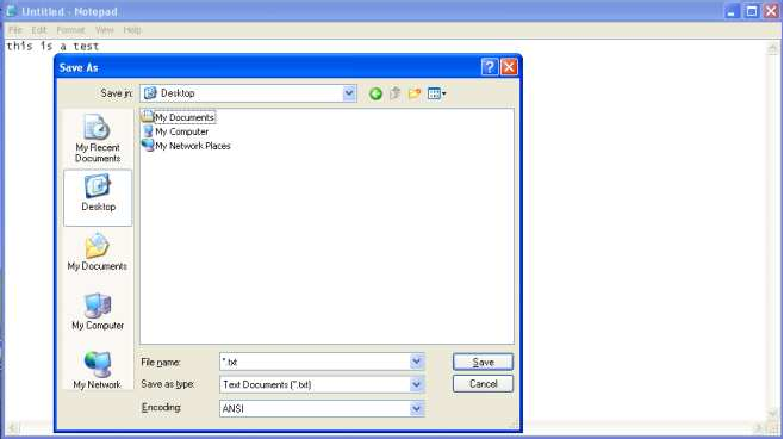
\includegraphics[width=65mm]{images/figure17}
\end{center}
%\caption{The save dialog from Windows Notepad.}\label{fig17}
\caption{Der Speichern Dialog im Windows Notepad.}\label{fig17}
\end{figure}

%Open the Python console again, and try the following:
Nun kannst du die Python Konsole wieder öffnen und folgendes eintippen:

%\begin{Verbatim}[frame=single]
%>>> f = open('c:\\test.txt')
%>>> print(f.read())
%\end{Verbatim}
\begin{Verbatim}[frame=single]
>>> f = open('c:\\test.txt')
>>> print(f.read())
\end{Verbatim}

%The contents of the file you just created should be printed to the console. You can now jump ahead to the bit that says: ``Continuing from here$\ldots$''.
Der Inhalt der Datei die du eben erzeugt und gespeichert hast, sollte auf der Konsole ausgegeben werden. %Nun kannst du dem Teil springen wo steht: ``Hier gehts weiter$\ldots$''.
\end{WINDOWS}

\begin{MAC}
%To see how \code{file} is used, open up the Text Editor, by clicking on the editor icon (\includegraphics*[width=12mm]{textedit-icon.eps}).  Type a few words then save the file to the Desktop by clicking File, then Save, and entering the name `text.txt' in the entry box next to `Save As'.
Um zu sehen wie du \code{file} verwenden kannst, öffne den Text Editor, indem du auf das icon (\includegraphics*[width=12mm]{images/textedit-icon}) klickst. Gib ein paar Worte ein und speichere die Datei auf dem Desktop indem du im Menü auf File klickst, dann auf Speichern und den Namen `text.txt'  neben dem `Speichern unter' Feld eingibst.

\begin{figure}
\begin{center}
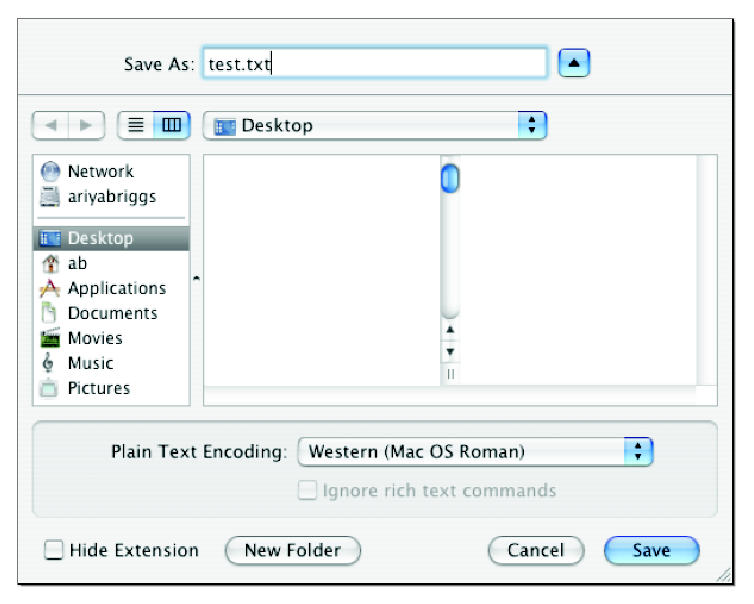
\includegraphics[width=65mm]{images/figure18}
\end{center}
%\caption{The save dialog from Mac OS X Text Editor.}\label{fig18}
\caption{Der speichern Dialog vom Mac OS X Text Editor.}\label{fig18}
\end{figure}

%Open the Python console again, and try the following:
Nun kannst du die Python Konsole wieder öffnen und folgendes eintippen:

%\begin{Verbatim}[frame=single]
%>>> f = open('Desktop/test.txt')
%>>> print(f.read())
%\end{Verbatim}
\begin{Verbatim}[frame=single]
>>> f = open('Desktop/test.txt')
>>> print(f.read())
\end{Verbatim}

Falls es nicht funktioniert, könnntest du den ganzen Pfad zur Datei direkt angeben. Zum Beispiel:

\begin{Verbatim}[frame=single]
>>> f = open('/Users/Benutzername/Desktop/test.txt')
>>> print(f.read())
\end{Verbatim}

%The contents of the file you just created should be printed to the console.  You can now jump ahead to the bit that says: ``Continuing from here$\ldots$''.
Der Inhalt der Datei die du eben erzeugt und gespeichert hast, sollte auf der Konsole ausgegeben werden. %Nun kannst du dem Teil springen wo steht: ``Hier gehts weiter$\ldots$''.
\end{MAC}

\begin{LINUX}
%To see how \code{file} is used, open a text editor, type a few words and then save the file to your home directory, by clicking File, Save, selecting `Home Folder' (or `Home Directory' or `Home') and typing `test.txt' in the file name box (see figure~\ref{fig19} for an example).
Um zu sehen wie du \code{file} verwenden kannst, öffne einen Text Editor, tippe ein paar Worte ein und speichere die Datei dann auf deinem Desktop. Gehe im Menü auf Datei, `Speichern unter' und wähle Desktop. Als Dateinamen tippst du `test.txt' und gehst dann auf speichern (siehe Abbildung~\ref{fig19} als Beispiel).

\begin{figure}
\begin{center}
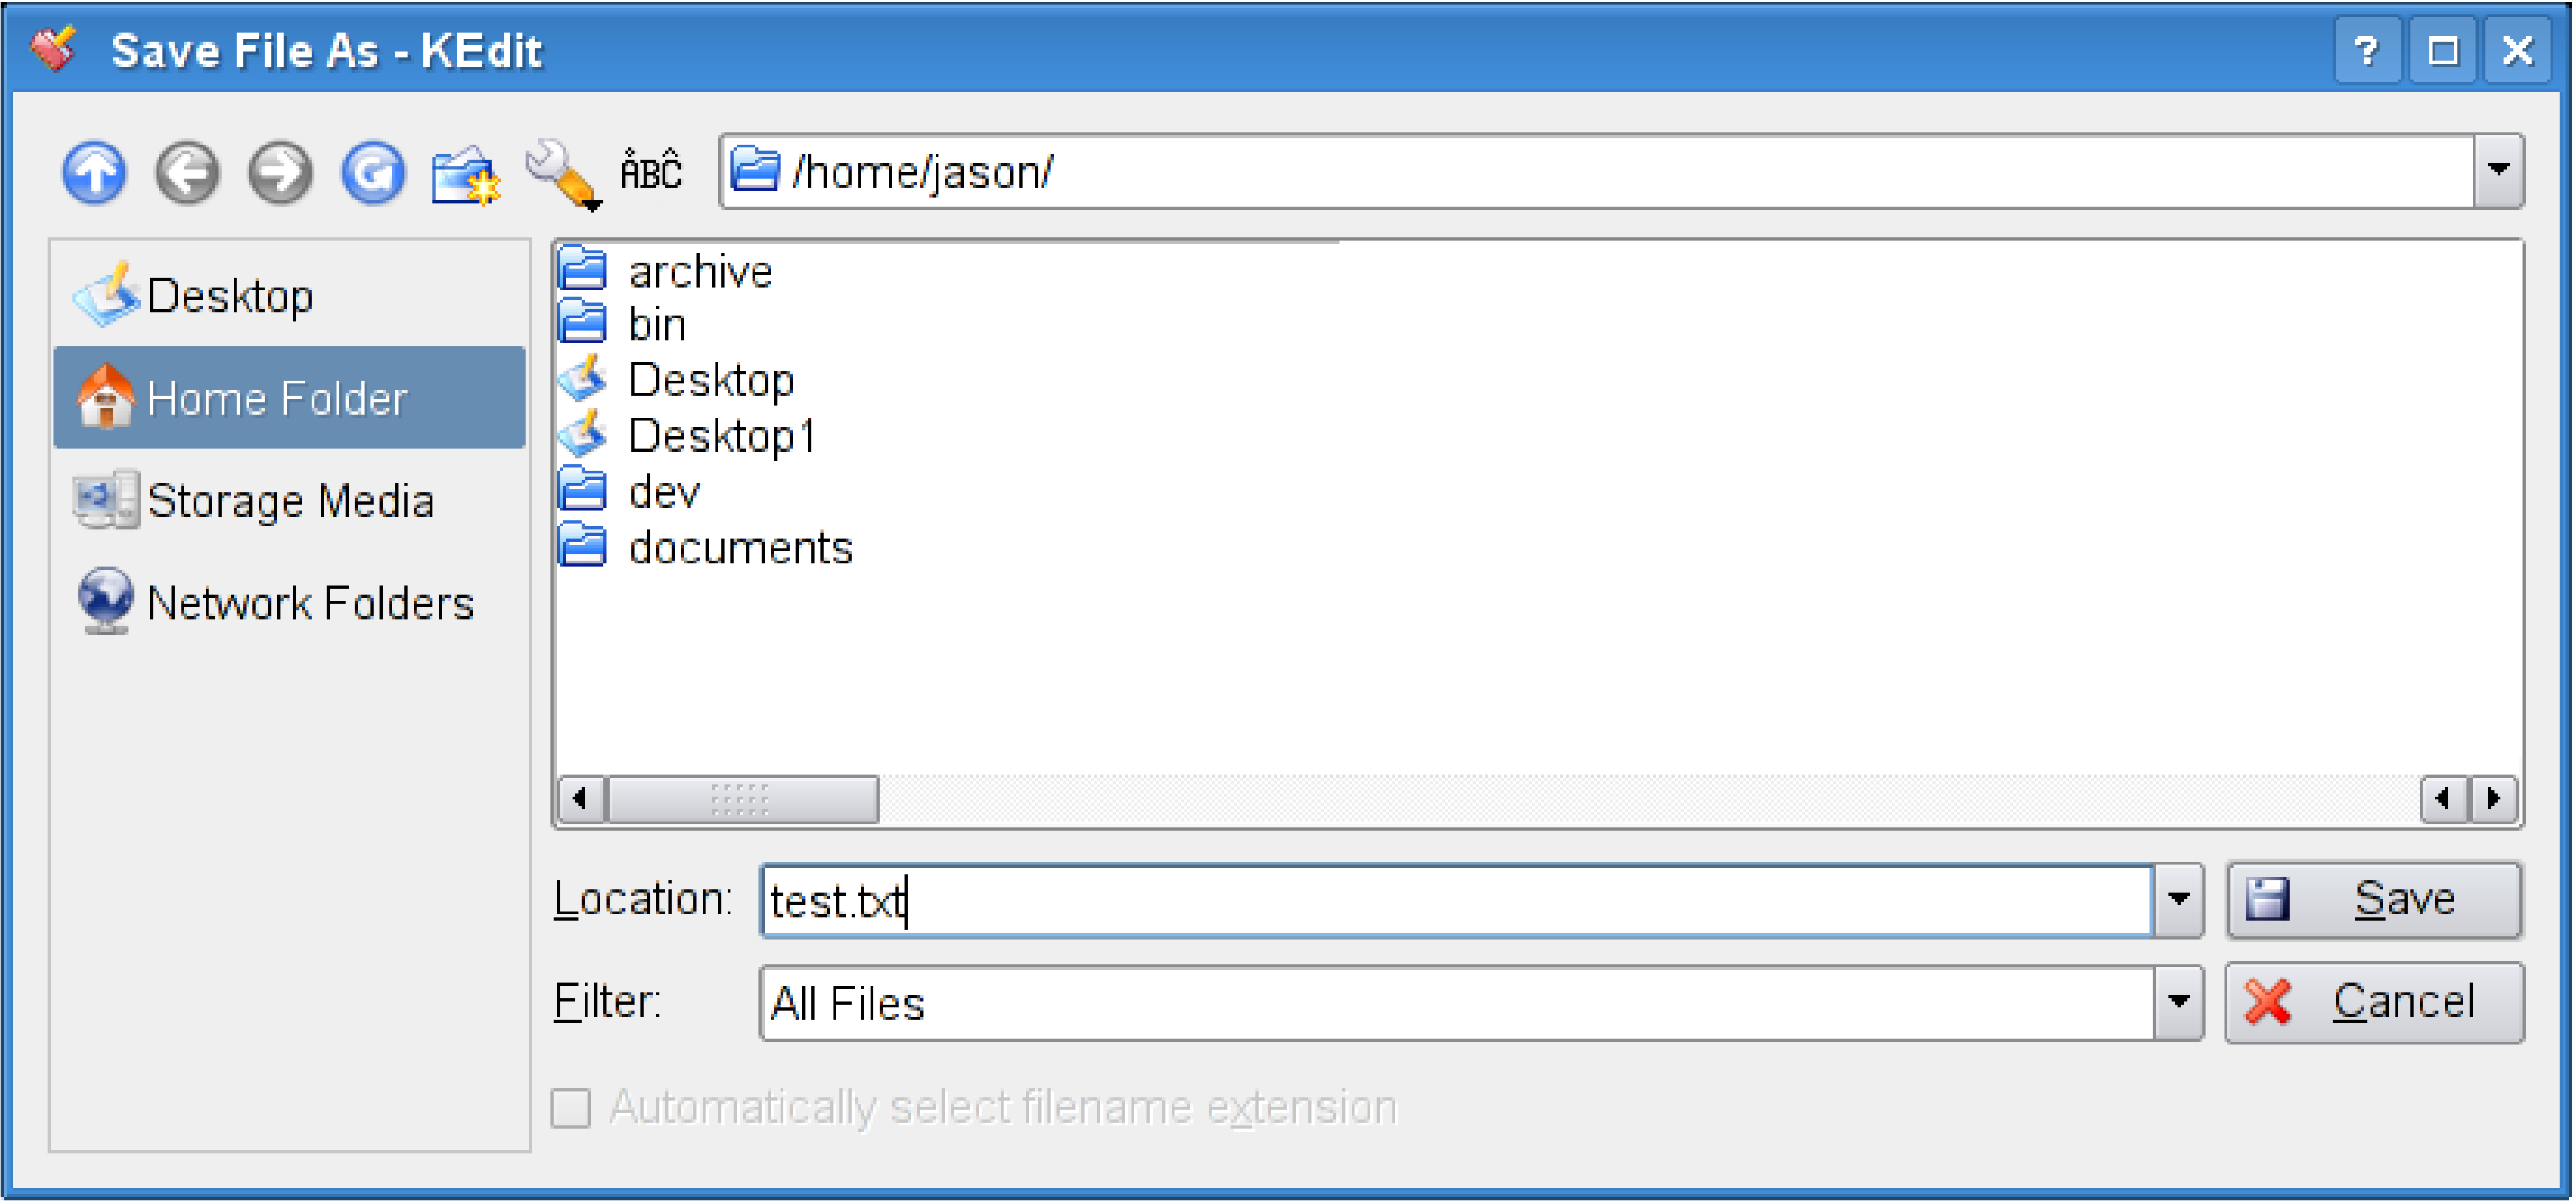
\includegraphics[width=65mm]{images/figure19}
\end{center}
%\caption{The save dialog from the KEdit Text Editor.}\label{fig19}
\caption{Der Speichern Dialog vom KEdit Texteditor.}\label{fig19}
\end{figure}

%Open the Python console again, and try the following:
Nun kannst du die Python Konsole wieder öffnen und folgendes eintippen:

%\begin{Verbatim}[frame=single]
%>>> f = open('Desktop/test.txt')
%>>> print(f.read())
%\end{Verbatim}
\begin{Verbatim}[frame=single]
>>> f = open('Desktop/test.txt')
>>> print(f.read())
\end{Verbatim}

Der Inhalt der Datei die du eben erzeugt und gespeichert hast, sollte auf der Konsole ausgegeben werden. %Nun kannst du dem Teil springen wo steht: ``Hier gehts weiter$\ldots$''.
\end{LINUX}

%So what does that little bit of code do?  The first line calls the function \code{file}, passing the name of the file you just created, as a parameter.  The function returns a special type of value (called an object) which represents that file.  It's not the file itself; rather it's a bit like a big finger pointing at the file going ``HERE IT IS!!!!''  The file object is stored in the variable \code{f}.
Was macht denn nun dieser kurze Code? Die erste Zeile ruft die Funktion \code{file} auf und übergibt als Parameter den Dateinamen. Die Funktion gibt eine spezielle Variable (Objekt genannt) zurück, was die Datei darstellt. Es ist nicht die Datei selber. Es ist mehr wie ein Finger der auf die Datei zeigt und sagt ``DA IST ES!!!'' Das File Objekt (Datei Objekt) ist in der Variable \code{f} gespeichert.

\par
%The next line calls a special function (\code{read}) on the file object, to read in the contents of the file, and print the result to the console.  Because the variable \code{f} contains an object, this means we need to call the read function using the dot symbol (.).
Die zweite Zeile ruft die spezielle Funktion \code{read} auf um den Inhalt der Datei zu lesen und mit der \code{print} Funktion auszugeben. Da die Variable \code{f} das Datei Objekt enthält, wird die \code{read} Funktion auf die \code{f} Variable angewendet indem ein Punkt hinter das Objekt geschrieben wird.

\fbox{\colorbox{PaleBlue}{\parbox{.75\linewidth} {
\par
%Appendix~\ref{app:builtinfunctions} (at the back of this book) has more information about the functions that are built into Python.
Anhang~\ref{app:builtinfunctions} (am Ende diese Buches) listet die wichtigsten Python Funktionen auf.
\par
}}}

%\section{Modules}\index{modules}
\section{Module}\index{Module}

%We've actually seen a couple of different ways to reuse code already. One is a standard function, which we can create ourselves, or use the functions built into Python (like \code{range} and \code{file} and \code{int} and \code{str}). Another is a special kind of function on objects---which we can call using the dot symbol---and the next are modules; which are a way of grouping lots of functions and objects together in useful ways. An example of this is the module `time'\index{modules!time}:
Jetzt haben wir schon einige Varianten gesehen, wie man Code wieder verwenden kann. Eine davon ist eine selber angelegte Funktion zu verwenden oder eine bereits in Python eingebaute Funktion (wie \code{range}, \code{file} oder \code{str}). Eine andere Variante ist spezielle Funktionen auf Objekte anzuwenden---indem wir einen Punkt hinter das Objekt schreiben. Und die nächste Variante wäre die Verwendung von Modulen wie zum Beispiel das `time'\index{Module!time}:

%\begin{Verbatim}[frame=single]
%>>> import time
%\end{Verbatim}
\begin{Verbatim}[frame=single]
>>> import time
\end{Verbatim}

%The import command is used to tell Python we want to access a module.  In the above example, we're saying we want to use the `time' module. We can then call functions and objects that are available in this module, using the dot symbol yet again:
Mit dem Import Kommando sagen wir Python, dass wir ein Modul verwenden wollen. Im obigen Beispiel wird das Modul `time' eingebunden. Danach können wir Funktionen und Objekte verwenden, die in diesem Modul enthalten sind, indem wir wieder das Punkt Symbol verwenden:

%\begin{Verbatim}[frame=single]
%>>> print(time.localtime())
%(2006, 11, 10, 23, 49, 1, 4, 314, 1)
%\end{Verbatim}
\begin{Verbatim}[frame=single]
>>> print(time.localtime())
time.struct_time(tm_year=2010, tm_mon=1, tm_mday=1, tm_hour=17, tm_min=39, 
tm_sec=51, tm_wday=4, tm_yday=1, tm_isdst=0)
\end{Verbatim}

%localtime\index{modules!time!localtime} is a function \emph{inside} the module time, that returns the current date and time, broken up into individual parts---year, month, day, hour, minute, second, day of the week, day of the year, and whether or not it's daylight savings (1 if it is, 0 if it isn't).  The individual parts are stored in a tuple (see \emph{Tuples and Lists} on page~\pageref{tuplesandlists}.  You can use another function in the time module to convert the datetime returned by localtime, into something a bit more understandable:
localtime\index{Module!Time!localtime} ist eine Funktion \emph{innerhalb} vom time Modul, welches das aktuelle Datum und die Zeit zurückgibt---aufgeteilt in Jahr, Monat, Tag, Stunde, Minute, Sekunde, Tag der Woche, Tag im Jahr und ob es Sommer oder Winterzeit ist. Die Werte sind in einem Tupel (schlag nach bei \emph{Tupel und Listen} auf Seite~\pageref{tuplesandlists}. Du kannst eine andere Funktion vom time Modul verwenden um die zurückgegebenen Werte verständlicher darzustellen.

%\begin{Verbatim}[frame=single]
%>>> t = time.localtime()
%>>> print(time.asctime(t))
%Sat Nov 18 22:37:15 2006
%\end{Verbatim}
\begin{Verbatim}[frame=single]
>>> t = time.localtime()
>>> print(time.asctime(t))
Fri Jan  1 17:53:14 2010
\end{Verbatim}

\noindent
%We can do that all in a single line if we wanted to:
Das kannst du auch alles in eine Zeile verpacken, wenn du magst:

%\begin{Verbatim}[frame=single]
%>>> print(time.asctime(time.localtime()))
%Sat Nov 18 22:37:15 2006
%\end{Verbatim}
\begin{Verbatim}[frame=single]
>>> print(time.asctime(time.localtime()))
Fri Jan  1 17:53:14 2010
\end{Verbatim}

%Suppose you want to ask for someone to enter a value. You can do this using a \code{print} statement and the module `\code{sys}'\index{modules!sys}---imported the same way we imported the \code{time} module:
Nehmen wir an, du wolltest jemanden um eine Tastatureingabe fragen. Fragen könntest du mit \code{print} und die Antwort könntest du mit dem `\code{sys}'\index{Module!sys} Modul verarbeiten---sys kannst du genau gleich wie das \code{time} Module einbinden:

%\begin{Verbatim}[frame=single]
%import sys
%\end{Verbatim}
\begin{Verbatim}[frame=single]
import sys
\end{Verbatim}

%Inside the sys module is an object called `stdin'\index{modules!sys!stdin} (short for standard input).  stdin has a rather useful method (or function) called \code{readline}---which is used to read a line of text someone types on the keyboard (up until the point when they press the Enter key).  You can test \code{readline}, by entering the following command in the Python console:
Im sys Modul gibt es ein Objekt mit dem Namen `stdin'\index{Module!sys!stdin} (englisch für standard input). In stdin gibt es die nützliche Methode (oder Funktion) mit dem Namen \code{readline}---was verwendet wird um eine Eingabe auf der Tastatur zu verarbeiten (die Eingabe wird durch die Eingabetaste beendet). Teste \code{readline} indem du folgendes in die Python Konsole eingibst:

%\begin{Verbatim}[frame=single]
%>>> print(sys.stdin.readline())
%\end{Verbatim}
\begin{Verbatim}[frame=single]
>>> print(sys.stdin.readline())
\end{Verbatim}

%If you then type some words, and press the Enter key, what you've typed will be printed to the console. Think back, for a moment, to the code we wrote earlier, using an if-statement:
Danach tippst du irgendwelche Wörter und drückst am Ende die Eingabetaste. Alles was du bis dahin eingegeben hast wird nochmals auf der Python Konsole ausgegeben. Denke nochmals kurz an das Beispiel mit der if-Schleife:

%\begin{Verbatim}[frame=single]
%if age >= 10 and age <= 13:
%    print('you are %s' % age)
%else:
%    print('huh?')
%\end{Verbatim}
\begin{Verbatim}[frame=single]
if alter >= 10 and alter <= 13:
    print('Du bist %s' % alter)
else:
    print('was?')
\end{Verbatim}

%Rather than creating the variable \code{age} beforehand, we can now ask someone to enter the value instead.  How about first turning the code into a function$\ldots$
Statt die Variable \code{alter} schon vorher zu erzeugen, fragen wir jemanden dass er sein Alter eingibt. Zuerst machen wir aus dem Code eine Funktion$\ldots$

%\begin{Verbatim}[frame=single]
%>>> def your_age(age):
%...     if age >= 10 and age <= 13:
%...         print('you are %s' % age)
%...     else:
%...         print('huh?')
%...
%\end{Verbatim}
\begin{Verbatim}[frame=single]
>>> def dein_alter(alter):
...     if alter >= 10 and alter <= 13:
...         print('Du bist %s' % alter)
...     else:
...         print('was?')
...
\end{Verbatim}

%Which can be called, by passing a number as the parameter value.  We'll test that it works properly, first:
Diese Funktion kannst du aufrufen indem du eine Zahl als Parameter mitgibst. Testen wir zuerst ob es richtig funktioniert:

%\begin{Verbatim}[frame=single]
%>>> your_age(9)
%huh?
%>>> your_age(10)
%you are 10
%\end{Verbatim}
\begin{Verbatim}[frame=single]
>>> dein_alter(9)
was?
>>> dein_alter(10)
Du bist 10
\end{Verbatim}

%Now we know there are no problems with our function, we can change the function to ask for a person's age instead:
Jetzt wissen wir, dass unsere Funktion funktioniert. Nun ändern wir die Funktion, damit sie nach dem Alter der Person fragt:

%\begin{Verbatim}[frame=single]
%>>> def your_age():
%...     print('Please enter your age')
%...     age = int(sys.stdin.readline())
%...     if age >= 10 and age <= 13:
%...         print('you are %s' % age)
%...     else:
%...         print('huh?')
%...
%\end{Verbatim}
\begin{Verbatim}[frame=single]
>>> def dein_alter():
...     print('Bitte gib dein Alter ein')
...     alter = int(sys.stdin.readline())
...     if alter >= 10 and alter <= 13:
...         print('Du bist %s' % age)
...     else:
...         print('was?')
...
\end{Verbatim}

%Because \code{readline()} returns what a person typed as text (in other words, a string), we need to use the function \code{int} to convert it to a number (this so it will work correctly in the if-statement---check \emph{What's the difference} on page~\pageref{whatsthedifference} for more information about this).  To try it for yourself, call the your\_age function without any parameters, then type some text when `Please enter your age' appears:
Weil \code{readline()} das eingetippte als Text zurückgibt (oder anders gesagt als string), müssen wird das zuerst mit Hilfe der Funktion \code{int} in eine Zahl verwandeln (damit die if-Abfrage richtig funktioniert). Schau unter \emph{Was ist der Unterschied} auf Seite~\pageref{whatsthedifference} für mehr Information darüber. Rufe zum Ausprobieren die Funktion dein\_alter ohne Parameter auf und gib etwas ein, wenn `Bitte gib dein Alter ein' dasteht:

%\begin{Verbatim}[frame=single]
%>>> your_age()
%Please enter your age
%10
%you are 10
%>>> your_age()
%Please enter your age
%15
%huh?
%\end{Verbatim}
\begin{Verbatim}[frame=single]
>>> dein_alter()
Bitte gib dein Alter ein
10
Du bist 10
>>> dein_alter()
Bitte gib dein Alter ein
15
was?
\end{Verbatim}

\noindent
%\emph{The important thing to note here is that even though you're typing in a number (in the above case 10 or 15), readline always returns a string.}
\emph[{Das wichtige zum Merken ist hier, dass obwohl du eine Zahl eingegeben hast (einmal 10 und einmal 15) readline immer einen String zurückgibt.}

\fbox{\colorbox{PaleBlue}{\parbox{.75\linewidth} {
%\code{sys} and \code{time} are just two of the many modules that are included with Python.  For more information on some (but not all) Python modules, see Appendix~\ref{app:afewpythonmodules}.
Die Module \code{sys} und \code{time} sind nur zwei von den vielen Modulen die bei Python dabei sind. Für mehr Information zu weiteren (aber nicht allen) Python Modulen schlage bitte bei Anhang~\ref{app:afewpythonmodules} nach.
}}}

%\section{Things to try}
\section{Probiere es aus}

%\emph{In this chapter we saw how to do recycling in Python; through the use of functions and modules.  We saw a little bit about the `scope' of variable, how variables outside of functions can be `seen' inside, whereas variables inside cannot be seen outside, and learned how to create our own functions using \code{def}}
\emph{In diesem Kapitel haben wir gesehen, wie Wiederverwertung mit Python funktionert; durch Verwenden von Funktionen und Modulen. Wir haben ein wenig den `scope' (Sichtbarkeit) von Variablen behandelt und wie Variablen ausserhalb von Funktionen innerhalb dieser Funktionen `gesehen' werden können. Unsere eigenen Funktionen haben wir mit \code{def} erzeugt.}

%\subsection*{Exercise 1}
\subsection*{Übung 1}
%In exercise 2 in Chapter~\ref{ch:againandagain}, we created a for-loop to work out the interest we might earn from \$100 over a period of 10 years.  That for-loop could easily be turned into a function.  Try creating a function which takes a starting amount, and a rate of interest.  You could call the function using code like:
In Übung 2 aus Kapitel~\ref{ch:againandagain} haben wir eine for-Schleife verwendet um die Zinsen zu berechnen, die wir aus 100 € über die Zeit von 10 Jahren bekommen würden. Diese for-Schleife lässt sich gut in eine Funktion verpacken. Versuche eine Funktion zu definieren, der man die Geldsumme und den Zinssatz mitgibt. Diese könntest du folgendermaßen aufrufen:

%\begin{Verbatim}[frame=single]
%calculate_interest(100, 0.03)
%\end{Verbatim}
\begin{Verbatim}[frame=single]
berechne_zinsen(100, 0.03)
\end{Verbatim}

%\subsection*{Exercise 2}
\subsection*{Übung 2}
%Take the function you've just created, and make it calculate interest for different periods---such as 5 years or 15 years.  Perhaps you could call it using code like:
Nimm die Funktion die du gerade geschrieben hast und passe sie so an, dass sie verschiedene Zeiträume als Paramter annimmt---wie 5 Jahre oder 15 Jahre. Der Aufruf der Funktion könnte so ausschauen:

%\begin{Verbatim}[frame=single]
%calculate_interest(100, 0.03, 5)
%\end{Verbatim}
\begin{Verbatim}[frame=single]
berechne_zinsen(100, 0.03, 5)
\end{Verbatim}

%\*subsection*{Exercise 3}
\subsection*{Übung 3}
%Perhaps rather than a simple function, where we pass in the values as parameters, we can make a mini-program which asks someone for the values (using the \code{sys.stdin.readline()} function).  In this case, we'll call the function without any parameters at all:
Vielleicht wäre es noch besser, wenn wir die Paramter zuerst von einem Nutzer abfragen. Also schreiben wir eine Funktion, das nach den Werten für die Geldsumme, Zinssatz und Zeitdauer fragt. In diesem Fall rufen wir die Funktion ohne Parameter auf:

%\begin{Verbatim}[frame=single]
%calculate_interest()
%\end{Verbatim}
\begin{Verbatim}[frame=single]
berechne_zinsen()
\end{Verbatim}

\noindent
%To create this mini-program requires a function that we haven't talked about yet: \code{float}. The \code{float} function is a bit like the \code{int} function, except it converts strings into what is called floating point numbers (which we discussed briefly in Chapter~\ref{ch:8multipliedby3.57}).  Floating point numbers are numbers with a decimal place (.), such as 20.3 or 2541.933.
Um dieses kleine Programm zu erstellen brauchst du die Funktion \code{float}. Wir haben sie noch nicht behandelt, aber sie macht was sehr ähnliches wie die \code{int} Funktion. Sie konvertiert strings aber nicht zu Ganzzahlen (Integer) sondert zu Fließkommazahlen (floating point number, wie in Kapitel~\ref{ch:8multipliedby3.57} erklärt). Fließkommazahlen sind Nummern mit Kommastellen wie 20.3 oder 2541.933.

\newpage
